\subsection{Komparator}
\label{Komparator}
%
Komparatorens formål er at kontrollere og sammenligne en analog inputspænding, på den ikke-inverterende terminal, med en kendt referencespænding, på den inverterende terminal. Er inputspændingen højere end referencespændingen, giver komparatoren et digitalt højt output. Omvendt, hvis inputspændingen er lavere end referencespændingen, giver komparatoren et digitalt lavt output. Grunden til at komparatoren implementeres er for at sammenligne outputtet fra differensforstærkeren, som kobles til den ikke-inverterende input terminal på komparatoren, med jord, som kobles til den inverterende terminal. På den måde vurderer komparatoren om der er blevet skruet op eller ned for anlægget, inden signalet behandles af dobbeltensretteren. Outputtet fra komparatoren sendes videre til en multiplekser, og afhængigt af komparatorens output vælges der enten de filtre der forstærker de lave frekvenser eller de filtre der dæmper de lave frekvenser.  
%
\begin{figure}[H]
	\centering
	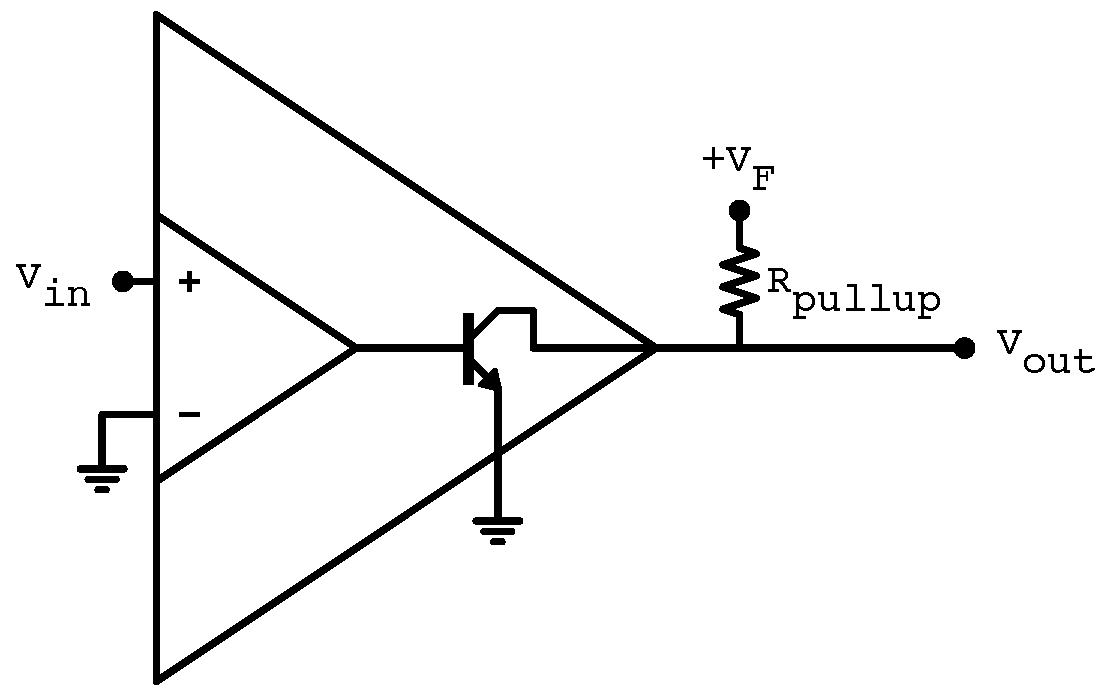
\includegraphics[resolution=300,scale=\circuitSize]{Figure/Circuits/Komparator_Internals.pdf}
	\caption{Kredsløbsdiagram for en komparator med en $pullup$ modstand.}
	\label{fig:Komparator}
\end{figure}
\noindent
%
Selvom det på \autoref{fig:Komparator} illustrerer at en komparator består af en operationsforstærker, så er det vigtigt at slå fast at det ikke er en almindelig operationsforstærker. Derimod er det en operationsforstærker, som er designet til komme langt hurtigere ud af mætning end almindeligvist. Ydermere består en komparator også af en transistor, hvis emitter er koblet til jord og kollektor er koblet til outputtet af komparatoren. Transistoren fungerer som en form for \textit{ON}/\textit{OFF} funktion, så når transistoren er \textit{ON} så vil outputtet på komparatoren være digitalt lavt, 0V, svarende til at inputspændingen er lavere end komparatorens referencespænding, som er jord. Hvis det er tilfældet vil de filtre, der forstærker de lave frekvenser, blive valgt. 

Hvis transistoren derimod er \textit{OFF}, så sørger $R_{pullup}$ for at komparatorens output bliver digitalt højt, da der ellers ikke løber en strøm. Udover at $R_{pullup}$ er koblet til komparatorens output, så kobles modstanden også til den positive forsyningsspænding, $+V_F$, som er fastlagt til +5V. Hvis det er tilfældet så vil de filtre, der dæmper de lave frekvensewr, blive valgt. \\[5mm]
%
I tilfældet hvor inputspændingen er meget tæt på eller lig med referencespændingen vil det resultere i at komparatorens output oscillerer mellem at være digitalt lavt eller digitalt højt. Der forekommer derfor et grænseområde omkring referencespændingen hvor komparatoren foretager systematiske fejl, jævnfør \autoref{fig:Hysterese}. 
%
\begin{figure}[H]
	\centering
	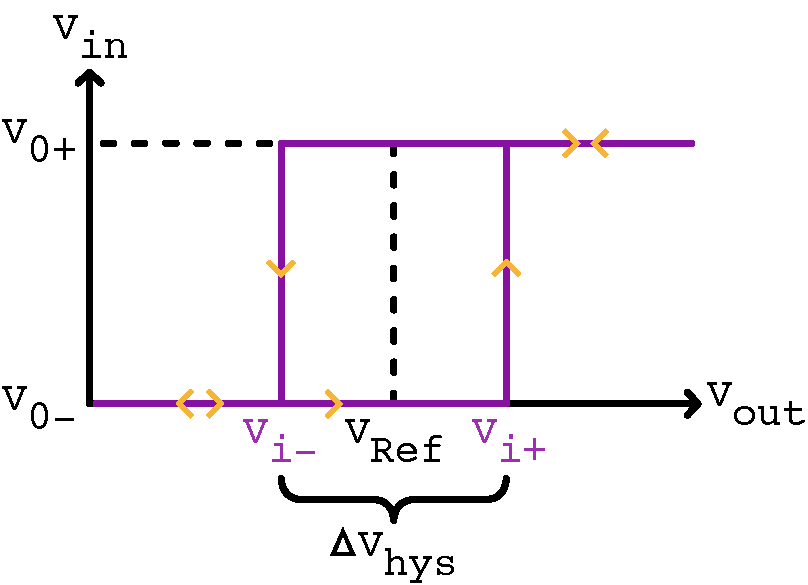
\includegraphics[resolution=300,scale=\circuitSize]{Figure/Circuits/Hysterese.pdf}
	\caption{Illustration af komparatorens oscillation, som forekommer når inputspændingen og referencenspændingen er tilnærmelsesvist ens.}
	\label{fig:Hysterese}
\end{figure}
\noindent
%
Fejlene, illustreret på \autoref{fig:Hysterese}, kan elimineres ved hjælp af hysterese, som er en positiv tilbagekobling mellem komparatorens input og output. Hysteresen definerer to tærskler, én for hvornår komparatoren giver et digitalt højt output og én for hvornår komparatoren giver et digitalt lavt output. På den måde vil komparatorens output ikke oscillerer, men være stabilt. 
%
\begin{figure}[H]
	\centering
	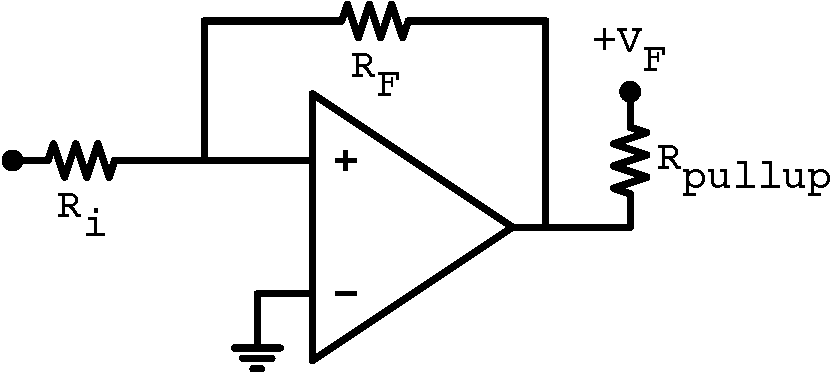
\includegraphics[resolution=300,scale=\circuitSize]{Figure/Circuits/Komparator_Hysterese.pdf}
	\caption{Kredsløbsdiagram for opkoblingen af komparatoren med hysterese, og $R_{pullup}$.}
	\label{fig:Komparator_Hysterese}
\end{figure}
\noindent
%
På \autoref{fig:Komparator_Hysterese} illustreres det, hvordan hysteresen inkluderes i den positive tilbagekobling. Som tidligere nævnt består hysterese af to tærskler; en der sørger for at outputtet bliver digitalt højt og en der sørger for at outputtet bliver digitalt lavt, det er så differencen mellem de to tærskler der udgør hysteresen. Den øvre tærskel, $V_{i+}$, er tærsklen for hvornår outputtet bliver digitalt højt, og har følgende overføringsfunktion:
%
\begin{equation}
	V_{i+} = V_{ref}*\left(1+\frac{R_i}{R_F}\right)-V_{o-}*\frac{R_i}{R_F}
\end{equation}
%
Hvor $V_{ref}$ er komparatorens referencespænding, som er koblet til jord og $V_{o-}$ angiver den spænding, som outputspændingen fra komparatoren skal være over, for at få et digitalt højt output.

Den nedre tærskel, $V_{i-}$, er tærsklen for hvornår outputtet bliver digitalt lavt, og har følgende overføringsfunktion:
%
\begin{equation}
	V_{i-} = V_{ref}*\left(1+\frac{R_i}{R_F}\right)-V_{o+}*\frac{R_i}{R_F}
\end{equation}
%
Hvor $V_{o+}$ angiver den spænding, som outputspændingen fra komparatoren skal være under, for at få et digitalt lavt output. 

For at beregne hysteresen, findes differencen mellem $V_{i+}$ og $V_{i-}$, hvilket gøres ved følgende udtryk:
%
\begin{equation}
	V_{i+}-V_{i-} = -V_{o-}*\frac{R_i}{R_F}+V_{o+}*\frac{R_i}{R_F} = \Delta V_{out}*\frac{R_i}{R_F}
\end{equation}
%
Hvilket kan omskrives til følgende udtryk:
%
\begin{equation}
	(V_{i+}-V_{i-}) = V_{hys} = (V_{o+}-V_{o-})*\frac{R_i}{R_F}
\end{equation}
%
Så divideres der med $\pm V_o$ for at separere modstandene fra spændingerne:
%
\begin{equation}
	\frac{R_F}{R_i} =\frac{V_{o+}-V_{o-}}{V_{i+}-V_{i-}} \Rightarrow \frac{R_F}{R_i} = \frac{\Delta V_{out}}{\Delta V_{hys}}
	\label{equ:BeregningAfHys}
\end{equation}
%
$\Delta V_{out}$ er den maksimale spænding komparatoren kan trække det digitale høje output op til, hvilket svarer til den positive forsyningsspænding, $+V_F$ på +5V. Hysteresen $\Delta V_{hys}$ vælges til 100mV baseret på hvor stor en spænding AD-konverteren skal bruge for at ændre den mindst betydende bit. Selvom det kun er de fire mest betydende bits, der anvendes i kredsløbet, så vil en lille spændingsstigning på den mindst betydende bit resulterer i at filtrene skifter uregelmæssigt. Derfor skal $\Delta V_{hys}$ vælges til en spænding der er højere end hvad der aktiverer den mindst betydende bit og lavere end den spænding der skal bruges til at aktivere den første af de fire bits der benyttes i kredsløbet, $\approx 320mV$, hvilket blev uddybet yderligere i \fullref{ADKonverter}.
%
\begin{figure}[H]
	\centering
	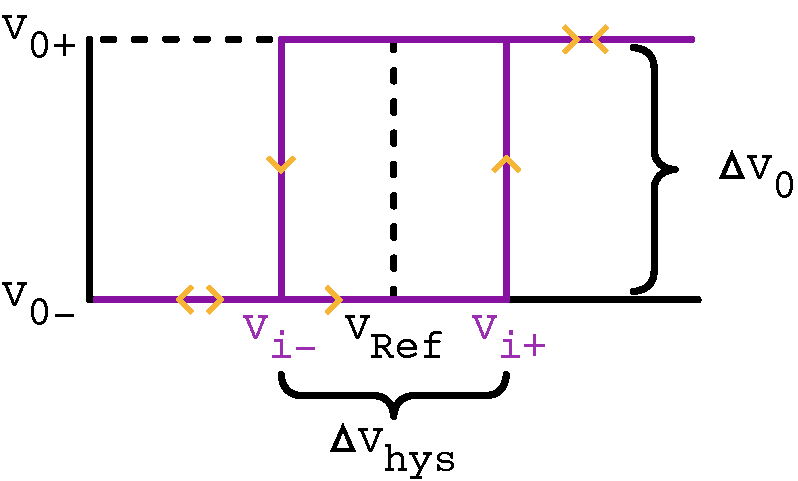
\includegraphics[resolution=300,scale=\circuitSize]{Figure/Circuits/Hysterese2.pdf}
	\caption{Repræsentation af hysterese, hvor det illustreres hvordan $V_{i-}$ og $V_{i+}$ skifter stadie afhængigt af $V_{in}$ og hvordan $V_{o-}$ og $V_{o+}$ skifter stadig afhængigt af $V_{out}$.}
	\label{fig:Komparator_Hysterese2}
\end{figure}
\noindent
%
På \autoref{fig:Komparator_Hysterese2} fremstilles en grafisk repræsentation af hysterese, hvor det tydeliggøres at afstanden mellem $V_{i-}$ og $V_{i+}$ gengiver hysteresen, $\Delta V_{hys}$. $V_{i-}$ og $V_{i+}$ er grænserne for hvornår outputtet skifter fra højt til lavt, eller omvendt. \\[5mm] 
%
Indgangsmodstanden $R_i$ og $R_{pullup}$ vælges begge til $10k\Omega$. Baseret på \autoref{equ:BeregningAfHys} er det muligt at dimensionere tilbagekoblingsmodstanden $R_F$, ved at isolere $R_F$ i udtrykket:
%
\begin{equation}
 \frac{R_F}{R_i} = \frac{\Delta V_{out}}{\Delta V_{hys}} \Rightarrow R_F = \frac{\Delta V_{out}}{\Delta V_{hys}*R_i}
\end{equation}
%
Ved at indsætte de kendte værdier beregnes $R_F$:
%
\begin{equation}
  R_F = \frac{5V}{100mV*10k\Omega} = 500k\Omega
\end{equation}
%
Komparatoren der er implementeret i kredsløbet er af typen LM311, som skal have den samme positive forsyningsspænding, som der er brugt andre steder i kredsløbet, nemlig $+V_F$ der er 5V. Databladet til LM311 fremgår af \textcite{PDF:Komparator}. Den maksimale inputspænding IC'en kan håndtere er $\pm 15V$, hvilket er en større spænding end hvad differensforstærkeren maksimalt kan levere som output. 







